\chapter{Security of IP Networks}
\begin{minipage}{0.6\textwidth}
%	\vspace{-0.5cm}
In IP networks, security’s main goal is to \textbf{control} who can \textbf{access} the network. In the past,
to make this possible, there were some devices called \textbf{Network Access Server (NAS)}, who’s tasks were: 
\begin{itemize}
    \item Perform \textbf{user's authN}.
    \item Perform \textbf{access control}.
    \item Eventually, provide to the user access to the IP network.
\end{itemize}
\end{minipage} 
\hspace{0.3cm}
\begin{minipage}{0.4\textwidth}
    \centering
    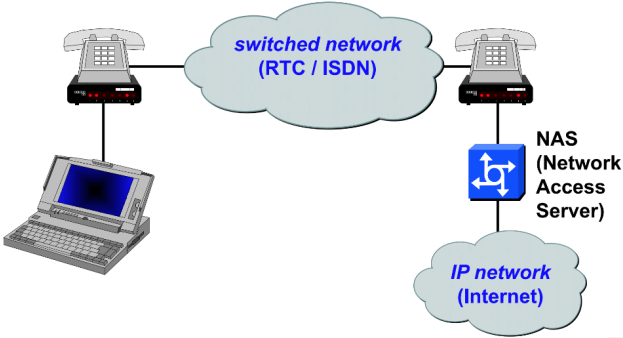
\includegraphics[width=\textwidth]{/home/lorenzo/Notes/Information System Security/images/Screenshot from 2024-12-29 17-23-09.png}
\end{minipage}
\\
\\
\noindent
\begin{minipage}{0.6\textwidth}
	\vspace{-2cm}
Nowadays, this scheme is not used anymore, as it is possible to access Internet in different
ways depending on the device. Independently of how the user decides to access the network,
user authN must always be performed before allowing any traffic from that user. 
\end{minipage} 
\hspace{0.4cm}
\begin{minipage}{0.4\textwidth}
    \vspace{0.3cm}
    \centering
    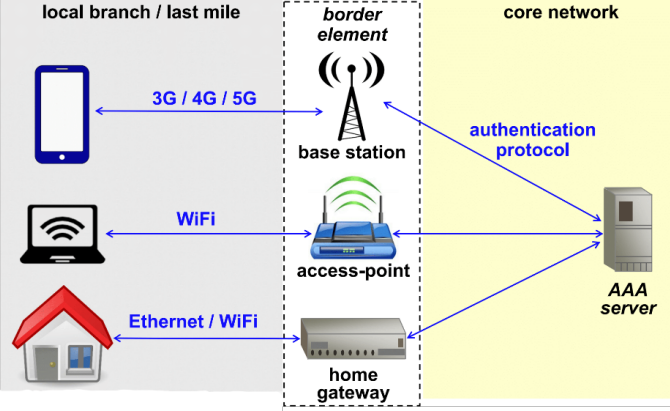
\includegraphics[width=0.9\textwidth]{/home/lorenzo/Notes/Information System Security/images/Screenshot from 2024-12-29 17-24-55.png}
\end{minipage}
\section{Authentication of PPP Channels}
There is the need to perform authN of the user \textbf{before} network transmission is enabled. Since
authN starts when someone is trying to connect, surely, the \textbf{physical} and \textbf{data layers} (L1 and L2) are already available.\\ The \textbf{Point-to-Point Protocol} (\textbf{PPP}) is a data link layer protocol (Layer 2 in the OSI model)
used for establishing direct connections between two network nodes. PPP is able to
encapsulate network packets and carry them over a point-to-point link (\(\rightarrow \)  there are many \textbf{Virtual PPP Links} going from one device to other Access Points).
\\ A \textbf{PPP link} is activated in three sequential steps:
\begin{itemize}
    \item \textbf{Link Establishment}: The devices at both ends of the link establish a connection, usually through signaling or negotiation protocols (\textbf{LCP - Link Control Protocol}).
    \item \textbf{Authentication}: If necessary (\textcolor{red}{\textbf{Optional}}), authentication takes place to verify the identity of the connecting devices, often using protocols like:
    \begin{itemize}
        \item Password Authentication Protocol (PAP)
        \item Challenge Handshake Protocol (CHAP)
        \item Extensible Authentication Protocol (EAP)
    \end{itemize} 
    \item \textbf{Network Layer Configuration}: L3 encapsulation is performed via various Network Control Protocols (NCPs), such as IP Control Protocol (IPCP) for IP packets, enabling data transfer to begin.
\end{itemize}
\newpage
\subsection{PAP (Password Authentication Protocol)}
The \textbf{oldest one}. In the case of \textbf{PAP}, the user sends username and password in \textbf{cleartext} over the PPP Link (\(\rightarrow \) authN happens \textbf{only} once the PPP Link is created, so sniffing and MITM attacks are possible).
\vspace{-0.4cm}
\begin{center}
\begin{quotebox-grey}{\textbf{PAP} uses a \textbf{2-way Handshake Protocol}:}
    \begin{enumerate}
        \item \textbf{Authenticate Request} (\textbf{Code = 1}), the peer sends to the authenticator the following packet:
        \begin{itemize}
            \item Code (8 bits) + Identifier (8 bits) + Length (16 bits)
            \item PeerID Length in bytes (8 bits) + PeerID (0-255 bytes)
            \item Password Length in bytes (8 bits) + Password (0-255 bytes)
        \end{itemize}
        \item \textbf{Authenticate Response} (\textbf{Code = 2, 3}), the authenticator sends to the peer the following packet:
        \begin{itemize}
            \item Code (8 bits) + Identifier (8 bits) + Length (16 bits), where:
            \begin{itemize}
                \item If the previous data was received correctly \(\rightarrow \) Code = 2 (ACK)
                \item Else \(\rightarrow \) Code = 3 (NAK)
            \end{itemize}
            \item Message Lenght in bytes (8 bits) + Message (0-255 bytes)
        \end{itemize}
    \end{enumerate}
\end{quotebox-grey}
\end{center}
\noindent
The Identifier \textbf{must} match between request and response. Moreover, the request or the response may be lost, so the authenticator \textbf{must} allow multiple requests from the same peer.

\subsection{CHAP (Challenge Handshake Authentication Protocol)}
\textbf{CHAP} uses a Symmetric CRA who’s response is based on the user’s password, the initial challenge is generated at the \textbf{creation} of the PPP Link (\(\rightarrow \) Sniffing attacks are not possible, but MITM attacks still are). CHAP is \textbf{safer} than PAP, so if an authenticator supports PAP and CHAP \(\rightarrow \) CHAP \textbf{must} be offered first.
\vspace{-0.4cm}
\begin{center}
\begin{quotebox-grey}{CHAP uses a \textbf{3-way Handshake Protocol}:}
    \begin{enumerate}
        \item \textbf{Challenge} (\textbf{Code = 1}), the authenticator sends to the peer the following packet:
        \begin{itemize}
            \item Code (8 bits) + Identifier (8 bits) + Length (16 bits)
            \item Challenge Size in bytes (8 bits) + Challenge (0-255 bytes)
        \end{itemize}
        \item \textbf{Response} (\textbf{Code = 2}), the peer sends to the authenticator the following packet:
        \begin{itemize}
            \item Code (8 bits) + Identifier (8 bits) + Length (16 bits)
            \item Response Size in bytes (8 bits) + Response (0-255 bytes), where:
            \[Response\ =\ MD5(Identifier\ ||\ Password\ ||\ Challenge)\]
        \end{itemize}
        \item \textbf{Result} (\textbf{Code = 3, 4}), the authenticator sends to the peer the following packet:
        \begin{itemize}
            \item Code (8 bits) + Identifier (8 bits) + Length (16 bits), where:
            \begin{itemize}
                \item If response was correct \(\rightarrow \) Code = 3
                \item Else \(\rightarrow \) Code = 4
            \end{itemize}
        \end{itemize}
    \end{enumerate}
\end{quotebox-grey}
\end{center}
\noindent
As in PAP, the Identifier \textbf{must} match between challenge and response. Moreover, the challenge or the response may be lost, so the authenticator \textbf{must} resend a \textbf{different} (nonce, random, non-invertible) challenge if no response arrives (up until the retry limit is hit).

\begin{customquote}
\vspace{-0.0cm}

\textbf{MS-CHAP} is the \textbf{Microsoft extension} of CHAP, every Windows system from Windows Vista to Win11 22H2 uses it. MS-CHAP has two official versions, v1 and v2:
\begin{itemize}
    \item \textbf{Common Traits}:
    \begin{itemize}
        \item Authenticator controlled password change.
        \item Authenticator controlled authN retry.
        \item Specific failure codes.
    \end{itemize}
    \item \textbf{v2 updates}: v2 provides \textbf{mutual authN} by piggybacking a peer challenge on the response and by adding an authenticator response on the Success packet.
\end{itemize}
\vspace{-0.4cm}
\begin{quotebox-red}{Beware}
    \textbf{MS-CHAPv2} should \textbf{never} be used! Since with just \(2^{56}\) operations (\(\sim\) 23 hours with DES
FPGA) we can decrypt the response \(\rightarrow \) critical security errors in the protocol.

\end{quotebox-red}
\end{customquote}

\subsection{EAP (Extensible Authentication Protocol)}
\textbf{EAP} is a flexible L2 authN framework, because \textbf{before} getting access to L3, \textbf{authN is required}. EAP does not implement any method, meaning that the authN method is external
(e.g. CRA, OTP, TLS, etc...). Still, some authN mechanisms are already predefined, such as: MD5-challenge, generic OTP and generic Token Card.\\    \\    
AuthN data are transported over L2 via a specific Encapsulation Protocol, which is needed because L3 is \textbf{not} available yet. \textbf{EAP Encapsulation} has the following features:
\begin{itemize}
    \item It is completely \textbf{indipendent} from IP.
    \item \textbf{ACK} and \textbf{NAK} are explicit.
    \item EAP assumes \textbf{no} reordering of the packets for transmission happening on PPP Links.
    \item Retransmission \textbf{must} be guaranteed for \textbf{at least} 3-5 times.
    \item \textbf{No} fragmentation by default.
\end{itemize}
In EAP, the PPP Link is \textbf{not} assumed secure \(\rightarrow \) EAP methods \textbf{must} provide security on their own. Some EAP methods are:
\begin{itemize}
    \item \textbf{EAP-TLS} \(\rightarrow \) for TLS Mutual AuthN.
    \item \textbf{EAP-MD5} \(\rightarrow \) only for EAP Client AuthN.
    \item \textbf{EAP-TTLS} \(\rightarrow \) tunneled TLS.
    \item \textbf{PEAP} \(\rightarrow \) for TLS tunnel protection on EAP method.
\end{itemize}
\begin{minipage}{0.3\textwidth}
%	\vspace{-0.5cm}
    EAP is supported by: 
    \begin{itemize}
        \item PPP
        \item 802.3 (Ethernet)
        \item 802.5 (Token Ring)
        \item 802.11 (Wi-Fi)
    \end{itemize}
\end{minipage} 
\hspace{0.3cm}
\begin{minipage}{0.4\textwidth}
    
    \includegraphics[width=0.8\textwidth]{/home/lorenzo/Pictures/Screenshots/Screenshot from 2024-12-30 10-12-19.png}
\end{minipage}
\\
\\
\noindent{\color{gray!50}\rule{\textwidth}{0.5pt}}
\section{Authentication for Network Access}
\begin{minipage}{0.5\textwidth}
%	\vspace{-0.5cm}
The process of authenticating users for network access, involving multiple components manage and verify permissions. The main components are:
\begin{itemize}
    \item \textbf{Network Access Server}
    \item \textbf{Protocol Manager} (\(\rightarrow \) acting as a intermediary, it handles the communication between NAS and the Authenticator Server)
    \item \textbf{Authentication Server}  (\textbf{AS}) 
\end{itemize}
\end{minipage} 
\hspace{0.3cm}
\begin{minipage}{0.5\textwidth}
    \centering
    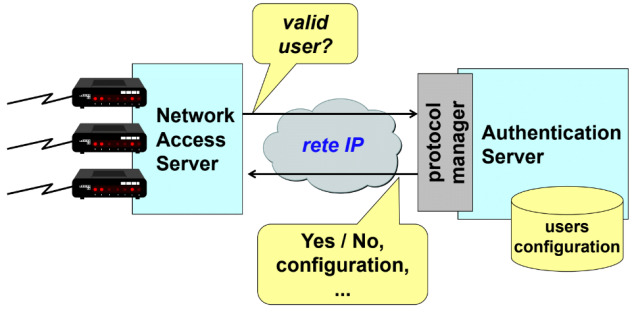
\includegraphics[width=0.9\textwidth]{/home/lorenzo/Notes/Information System Security/images/Screenshot from 2024-12-30 10-27-20.png}
\end{minipage}
\\
\\
\noindent
The devices that connect all the user of the LAN are controlled by a NAS.
The NAS will talk with the AS, which has access to a database that contains user credentials.
The AS will then respond to the NAS, providing the validity/invalidity of the user.\\
\noindent
NAS manufacturers claim that security needs to be implemented by the AS using \textbf{AAA}:
\begin{itemize}
    \item \textbf{Authentication}: a user’s identity is authN based on credentials.
    \item \textbf{Authorization}: determining whether an entity is authorized to perform a given activity or gain access to the resources or services.
    \item \textbf{Accounting}: tracking network resource usage for audit support, capacity analysis and cost billing;
\end{itemize}
\noindent
To communicate, NAS and AS can use three different \textbf{Network Authentication Protocols}:
\begin{itemize}
    \item \textbf{RADIUS}: it is the de-facto standard. RADIUS has a nice feature that makes it behave like a \textbf{proxy} towards other authN systems. It can be both an authN system and an external AS.
    \item \textbf{DIAMETER}: evolution of RADIUS, that takes better care of security.
    \item \textbf{TACACS+}: competitor of RADIUS, better but it is a proprietary solution of CISCO without any public specification.
\end{itemize}
\newpage
\subsection{RADIUS (Remote Authentication Dial-In User Service)}
\textbf{RADIUS} is a Client-Server Protocol between NAS and AS that uses port \textbf{1812/UDP} for
authN and port \textbf{1813/UDP} for accounting. Since UPD is \textbf{unreliable}, each transmission with RADIUS is subject to \textbf{timeout} and (if no ACK is received) retransmission. RADIUS also implements centralized administration and accounting to control network access.\\
\\
\begin{minipage}{0.5\textwidth}
	\vspace{-0.8cm}
The \textbf{RADIUS Server} can query a \textbf{Local RADIUS DB} that contains all the valid users.
If the user associated with the \textbf{NAS Access Request} is \textbf{not} registered in the Local DB,
the RADIUS Server could still be connected to another \textbf{Security Domain} (another DB) and perform authN through it \(\rightarrow \) the \textbf{RADIUS Server} will act as a \textbf{Proxy} for the authN part by redirecting the request to the appropriate AS. 
\end{minipage} 
\hspace{0.0cm}
\begin{minipage}{0.5\textwidth}
    \centering
    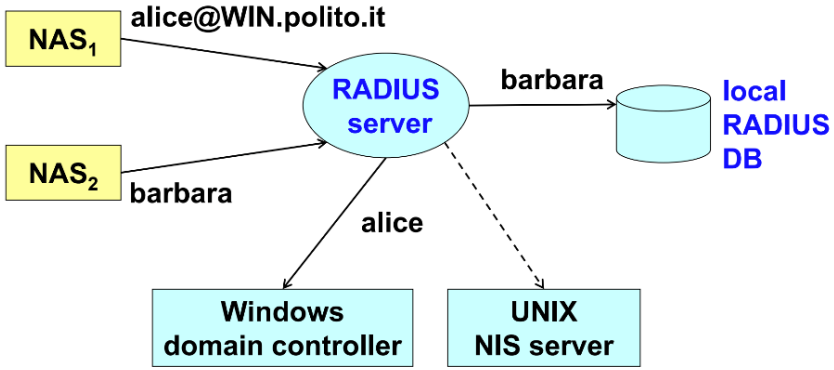
\includegraphics[width=0.9\textwidth]{/home/lorenzo/Notes/Information System Security/images/Screenshot from 2024-12-30 10-44-09.png}
\end{minipage}
RADIUS needs \textbf{security} functionalities to protect against:
\begin{itemize}
    \item \textbf{Sniffing NAS Requests}: if the NAS request contains a password in \textbf{cleartext} it could be sniffed, leading to privacy problems.
    \item \textbf{Fake AS Response}: an attacker could send an UDP packet before the actual AS, validating an unwanted user or blocking a valid one, causing a DoS attack. \textbf{Response authN} is required in this case.
    \item \textbf{Changing AS Response}: an AS response could be changed from valid to invalid or vice-versa. \textbf{Response authN} and \textbf{integrity} are required in this case.
    \item \textbf{Replay of AS Response}: An attacker might manipulate a legitimate
    AS response, altering the authentication result (e.g., changing a “No” to a “Yes” or vice versa) \(\rightarrow \) a User Identifier \textbf{must} be included in the response.
    \item \textbf{Password Enumeration}: this attack can be performed by a Fake NAS that sends fake requests to the RADIUS Server. To avoid this, \textbf{NAS authN} is required.
    \item \textbf{DoS against RADIUS Server}: this attack can be performed by a Fake NAS that floods the RADIUS Server with a lot of requests until it becomes unavailable.
    \\ 
    \\NAS are configured with a list of RADIUS servers to contact \(\rightarrow \) if \textbf{no} response arrives
    after a timeout, the NAS assumes that the server is busy and will switch to the next one.
    The resistance to this attacks is proportional to the number of secondary servers that is
    possible to setup in the system;
\end{itemize}
For \textbf{data protection} RADIUS uses \textbf{Keyed-Digest MD5} to gain \textbf{data integrity} and \textbf{data authN}:
\begin{itemize}
    \item The key is \textbf{shared secret} between the RADIUS server and the NAS (\(\rightarrow \) inserting a
    Fake NAS in the network would lead in the \textbf{rejection} of its requests).
    \item In case a user sends its password in \textbf{cleartext} (e.g. with PAP) then the password would
    \textbf{automatically} be \textbf{obfuscated} using MD5:
    \[
    password\ \oplus\  MD5(key\ ||\ authenticator) 
    \]
\end{itemize}
\begin{center}
\begin{quotebox-yellow}{Radius TLV attribute format}
    The most important characteristic of RADIUS is that it is an \textbf{Extensible Protocol}: each packet carries some attributes described with the TLV (Type-Length-Value) attributes.
    This allows the introduction of new types without breaking compatibility. There are different type of TLV attributes:
    \vspace{0.1cm}
    \begin{itemize}
        \item \textbf{Type = 1 (User-Name)} \(\rightarrow \) value can be: text, network access identifier (NAI), DN (Distinguish Name).
        \item \textbf{Type = 2 (User-Password)} \(\rightarrow \) \(value\ =\ password \oplus md5(key\ ||\ Request Authenticator)\).
        \item \textbf{Type = 3 (Chap-Password)} \(\rightarrow \) value = user CHAP response (128 bit).
        \item \textbf{Type = 60 (Chap-Challenge)} \(\rightarrow \) value = challenge form the NAS to the user.
    \end{itemize}
        \vspace{0.1cm}
        \centering
        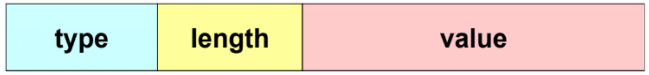
\includegraphics[width=0.5\textwidth]{/home/lorenzo/Notes/Information System Security/images/Screenshot from 2024-12-30 12-03-33.png}
\end{quotebox-yellow}
\end{center}
\vspace{0.0cm}
\noindent
\begin{minipage}{0.5\textwidth}
%	\vspace{-0.5cm}
    \textbf{RADIUS package} are formatted as follows:
    \begin{itemize}
        \item Code (8 bits)
        \item Identifier (8 bits)
        \item Length (16 bits)
        \item Authenticator (128 bits)
        \item TLV list of attributes
    \end{itemize} 
\end{minipage} 
\hspace{0.2cm}
\begin{minipage}{0.4\textwidth}
    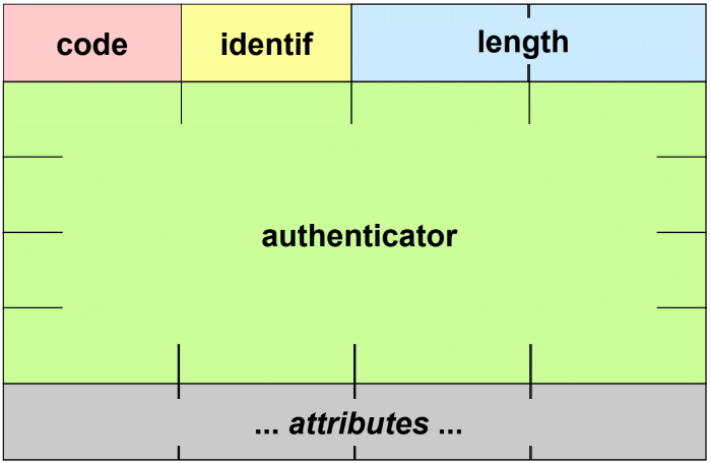
\includegraphics[width=0.7\textwidth]{/home/lorenzo/Notes/Information System Security/images/Screenshot from 2024-12-30 11-24-38.png}
\end{minipage}
\newpage
The RADIUS protocol defines various types of packets, for example:
\begin{itemize}
    \item \textbf{ACCESS-REQUEST} (NAS \(\rightarrow \) RADIUS): contains access credentials (e.g. username and password).
    \item \textbf{ACCESS-REJECT} (RADIUS \(\rightarrow \) NAS) : access is denied (e.g. bad username and/or password).
    \item \textbf{ACCESS-CHALLENGE} (RADIUS \(\rightarrow \) NAS): requests additional information from the user (e.g. PIN, tokenCode, etc...).
    \item \textbf{ACCESS-ACCEPT} (RADIUS \(\rightarrow \) NAS): access is granted and some networks parameters are given (e.g.
    IP address, netmask, MTU, port, etc...); 
\end{itemize}
\noindent
\vspace{-0.5cm}
\begin{quotebox-red}{Beware}
    Inside each packets there is an \textbf{Authenticator}, which has a double purpose:
    \begin{itemize}
        \item In the RADIUS Server Reply it provides \textbf{data authN} and protection from Replay attacks.
        \item It \textbf{masks} the password.
    \end{itemize}
    In the ACCESS-REQUEST, it is named \textbf{Request Authenticator} and it is a 16 bytes random value generated by the NAS. In the Server-Response (ACCESS ACCEPT/REJECT/CHALLENGE), it is named \textbf{Response Authenticator} and it is a \textbf{not} random value, which is computed via a Keyed-Digest MD5:
    \[
        MD5(Code\ ||\ ID\ ||\ Length\ ||\ Request\ Authenticator\ ||\ Attributes\ ||\ Secret)
    \]
\end{quotebox-red}

\begin{customquote}
\vspace{-0.4cm}
\subsubsection{NAI (Network Access Identifier)}
The \textbf{NAI} is used to distinguish requests coming form a local user, from requests coming from a user belonging to a \textbf{different} Security Domain. A \textbf{NAI} is defined as:\[ username[@realm]\]
\textbf{All} device \textbf{must} support NAI \textbf{up to} 72 bytes long.
\end{customquote}

\begin{center}
\begin{quotebox-grey}{Example: CHAP + RADIUS}
CHAP is used for \textbf{authN}, while RADIUS to \textbf{verify} the authN.\\
When the user connects to the system:
\begin{enumerate}
    \item The NAS sends a CHAP packet containing a Challenge Request.
    \item The user enters the password and provides the Challenge Response.
    \item The NAS does \textbf{not} posses the password \(\rightarrow \) it \textbf{cannot} verify the response \(\rightarrow \) the NAS will create a RADIUS ACCESS REQUEST packet containing:
    \begin{itemize}
        \item CHAP-Username
        \item CHAP-Challenge
        \item CHAP-Password
    \end{itemize}
    And it will then send it to the RADIUS Server.
    \item The RADIUS Server \textbf{verifies} the validity of the Challenge Response. Assuming that the
    response is good, the RADIUS Server sends to the NAS an \textbf{ACCESS-ACCEPT} packet containing the network parameters of the user.
    \item The NAS converts the received packet into a \textbf{CHAP-Success} packet and enables \textbf{L3
    Encapsulation} between NAS and user (e.g. with IPCP);
\end{enumerate}
    \vspace{0.2cm}
    \centering
    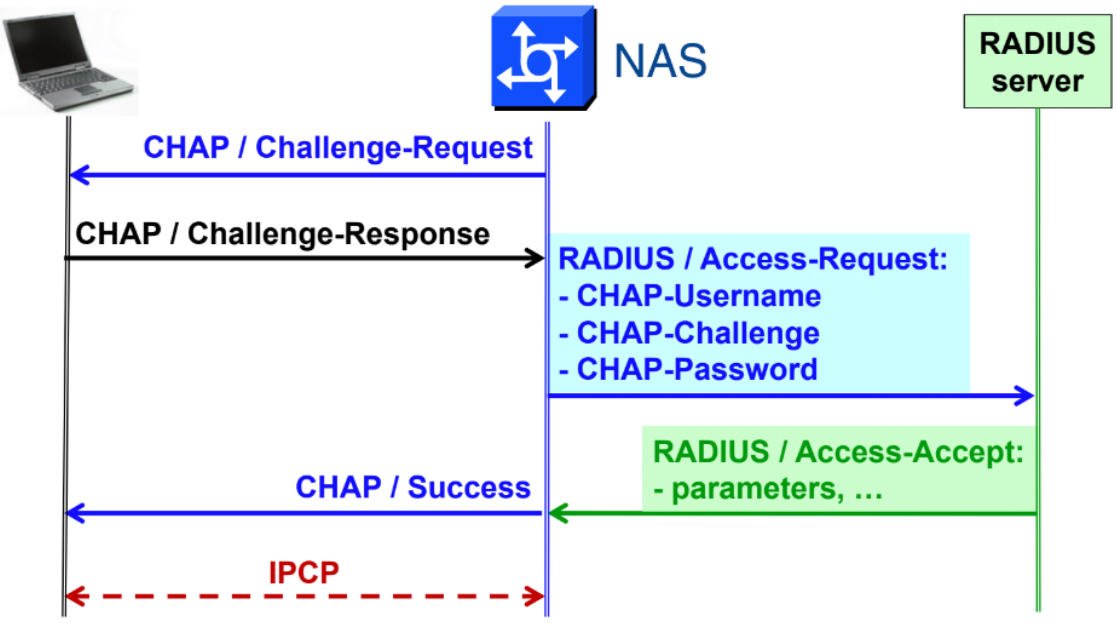
\includegraphics[width=0.5\textwidth]{/home/lorenzo/Notes/Information System Security/images/Screenshot from 2024-12-30 12-31-48.png}
\end{quotebox-grey}
\end{center}
\newpage
\section{IEEE 802.1x}
\textbf{802.1x} is an \textbf{AuthN Architecture} also known as \textbf{Port-Based Network Access Control}.
802.1x works at \textbf{L2} and \textbf{verifies} the identity and authorizations of users \textbf{before} letting them
communicate. 802.1x is \textbf{useful} in wired networks, but it is a \textbf{must} in \textbf{wireless} networks.\\    
\\    
802.1x is also an \textbf{authN} and \textbf{key-management framework} \(\rightarrow \) 802.1x does \textbf{not} impose a
specific authN solution, but it supports many of them. Key-management is needed for \textbf{wireless} networks as messages can be \textbf{easily sniffed}.\\    
\\ 
To protect wireless networks, 802.1x defines a Shared Symmetric Key that a \textbf{Supplicant} can use to \textbf{encrypt} traffic and \textbf{derive Session Keys} \(\rightarrow \) both used to achieve \textbf{data authN}, \textbf{integrity} and \textbf{confidentiality}.
%---------------------------------
\\ 
\\
\begin{minipage}{0.6\textwidth}
%	\vspace{-0.5cm}
In the picture above a \textbf{semi-public network} is represented. This network contains the devices that want to access the ISP network (the Supplicants). Meanwhile, the elements that reside
between this 2 networks are named \textbf{Authenticator} (or \textbf{EtherNAS}), which can be both Access Points or Switches.

802.1x allows Supplicants to connect to an EtherNAS using EAP in order to perform Client
AuthN. Depending on the type of EtherNAS the Supplicant communicates to, EAP is named:
\begin{itemize}
    \item \textbf{EAPOW} (\textbf{EAP Over Wireless}) \(\rightarrow \) if it is used over a \textbf{wireless} network.
    \item \textbf{EAPOL} (\textbf{EAP Over LAN}) \(\rightarrow \) if it is used over a \textbf{wired} network.
\end{itemize}
In the ISP network, there is \textbf{always} a RADIUS Server that performs \textbf{decapsulation} and \textbf{reencapsulation} of the packets to \textbf{verify} whether the user is a valid one or not. The connection between RADIUS Server and EtherNAS is \textbf{always} established with \textbf{EAPOR} (\textbf{EAP Over RADIUS}).
\end{minipage} 
\hspace{0.2cm}
\begin{minipage}{0.4\textwidth}
    \centering
    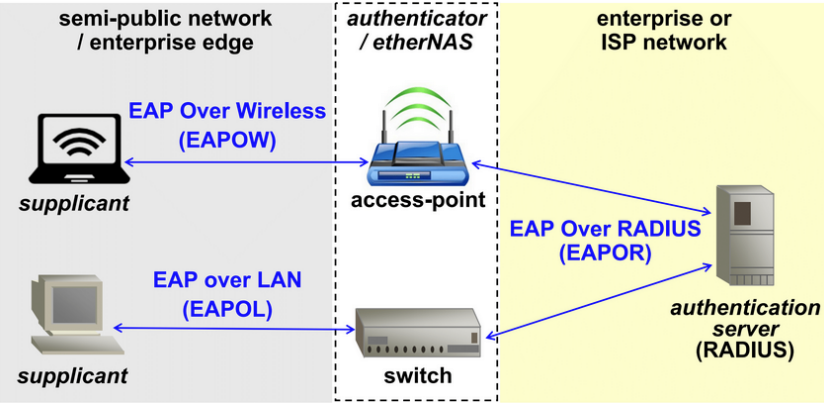
\includegraphics[width=\textwidth]{/home/lorenzo/Notes/Information System Security/images/Screenshot from 2024-12-30 14-17-20.png}
\end{minipage}
\\
\\
802.1x exploits the L7 for the actual implementation of the security mechanisms. There is a
direct dialogue between Supplicant and AS (Authentication Server = RADIUS Server) \(\rightarrow \)
the EtherNAS operates as a \textbf{pass-through device}, limiting its jobs to \textbf{ecapsulation} and \textbf{encapsulation}. \textbf{All} the authN mechanisms \textbf{must} be implemented \textbf{only} on the Supplicant and the RADIUS Server \(\rightarrow \) if authN mechanisms evolve in the future, the 802.1x architecture does \textbf{not} need to change.
\\
\\
\begin{minipage}{0.6\textwidth}
\vspace{-1.5cm}
In the above picture the Supplicant (laptop) wants to connect via EAPOL to the EtherNAS
(switch). To achieve this, the showed procedure is followed. If the second ACCESS-REQUEST
is valid, then the RADIUS server will provide a ACCESS-ACCEPT reply, which the EtherNAS
converts to an EAP Success reply. Now the Supplicant is considered a valid user of the network
and is allowed to communicate.
\end{minipage} 
\hspace{0.2cm}
\begin{minipage}{0.4\textwidth}
    \centering
    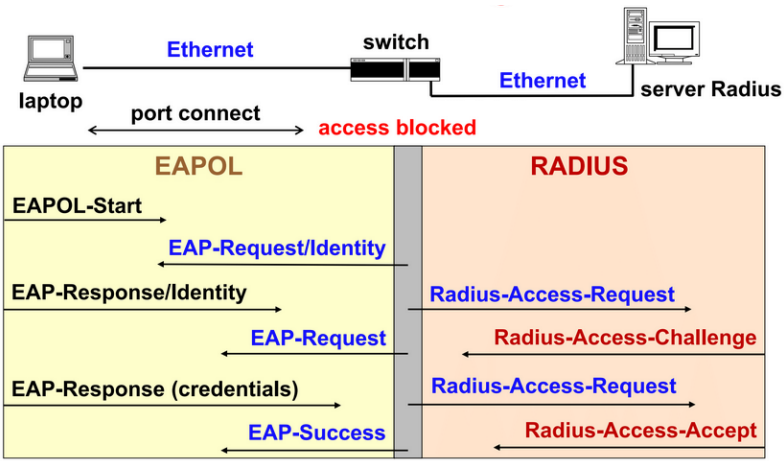
\includegraphics[width=\textwidth]{/home/lorenzo/Notes/Information System Security/images/Screenshot from 2024-12-30 14-46-16.png}
\end{minipage}
\begin{center}
\begin{quotebox-yellow}{Example}
    \hspace{-2.9cm}
    A major example of usage of 802.1x with RADIUS is the \textbf{eduroam} network:
    \\
    \\
        \centering
        \includegraphics[width=0.5\textwidth]{/home/lorenzo/Pictures/Screenshots/Screenshot from 2024-12-30 14-50-45.png}
\end{quotebox-yellow}
\end{center}